Language models are typically evaluated by the perplexity they assign to held out data, and thus did we evaluate our language models in the previous chapters. In this chapter we look at alternatives. In particular, we look at evaluation that specifically probes the syntactic abilities of a language model. To this end we take the dataset introduced by \citet{linzen2018targeted}, which presents a comprehensive set of syntactic challenges, and evaluate the models presented thus far against them. The dataset consists of constructed sentence pairs that differ in only one word, making one sentence grammatical and the other not. The task is to assign higher probability to the grammatical sentence. We can think of this task as soliciting comparative \textit{acceptability judgements}---a key concept in linguistics. We will refer to this dataset as Syneval, for \textit{syntactic evaluation}.

In this chapter:
\begin{itemize}
  \item We review the Syneval dataset: we describe syntactic phenomena that it tests and discuss how this dataset relates to other work on syntactic evaluation.
  \item We modify the training of standard RNN language model by adding a syntactic side objective, a form of multitask learning previously proposed to improve RNN language models on this task. We review a previously proposed approach that combines language modelling with CCG supertagging \citep{enguehard2017multitask}, and introduce a novel multitask language model based on span labeling inspired by the scoring function of our CRF parser.
  \item We evaluate all the models introduced thus far on this dataset and show that this gives finegrained differentation between the various models, generally favoring the RNNG, but often closely followed by and sometimes surpassed by the multitask models.
\end{itemize}

\section{Syntactic evaluation}
  A shortcoming of perplexity is that the metric conflates various sources of success \citep{linzen2018targeted}. A language model can make use of many aspects of language to predict the probability of a sequence of words. And although we would like the probability of a sentence to depend on high-level phenomena such as syntactic well-formedness or global semantic coherence, a language model can also focus on lower hanging fruit such as collocations and other semantic relations predicted from local context. Syntax is especially difficult to evaluate given that most sentences in a corpus are grammatically simple \citep{linzen2018targeted}. Arguably, this conflation is also the appeal: perplexity is a one size fits all metric. But for a fine-grained analysis we must resort to a fine-grained metric.

  Recently, a series of papers has introduced tasks that specifically evaluate the syntactic abilities of language models \citep{linzen2016syntax,gulordava2018colorless,linzen2018targeted}. And such tasks can be very revealing. The task introduced by \citet{linzen2016syntax} is to predict the correct conjugation of a verb given an earlier occuring subject---especially in the presence of distracting subjects that intervene\footnote{E.g. \textit{Parts} of the river valley \textit{have}/\textit{has}.}. This task has revealed that lower perplexity does not imply greater success on this task \citep{tran2018recurrent}, and that an explicitly syntactic model like the RNNG significanlty outperforms purely sequential models, especially with increasing distance between the subject and the verb \citep{kuncoro2018learn}. This type of agreement is one of the phenomena evaluated in Syneval.

  \subsection{Dataset}
    The Syneval dataset consists of contrastive sentence pairs that differ in only one word. Let $(\x, \x')$ be this minimal pair, with grammatical sentence $\x$ and an ungrammatical sentence $\x'$. Then a language model $p$ makes a correct prediction on this pair if $p(\x) > p(\x')$.

    The classification is based on the probability of the entire sequence. This makes the task applicable to grammatical phenomena that involve interaction between multiple words, or where the word of contention does not have any left context. This contrasts with the task introduced in \citet{linzen2016syntax}. This approach is also more natural for a model like the RNNG, where the probability of the sentence is computed by marginalizing over all latent structures, whereas individual word probabilities can only be obtained when conditioning on a single structure---for example a predicted parse---as is done in \cite{kuncoro2018learn}.

    The sentence pairs fall into three categories that linguists consider to depend crucially on hierachical syntactic structure \citep{everaert2015structures,xiang2009illusory}:
      \begin{enumerate}[noitemsep]
        \item Subject-verb agreement (The farmer \textit{smiles}.)
        \item Reflexive anaphora (The senators embarassed \textit{themselves}.)
        \item Negative polarity items (\textit{No} authors have \textit{ever} been famous.)
      \end{enumerate}
    The dataset contains constructions of increasing difficulty for each of these categories. For example, the distance between two words in a syntactic dependency can be increased by separating them with a prepositional phrase: \textit{The farmer next to the guards smiles}. In this example \textit{the guards} additionally forms a distractor for the proper conjugation of \textit{smiles}, making the example extra challenging. The dataset is constructed automatically using handcrafted context-free grammars. The lexical rules are finegrained so that the resulting sentences are semantically plausible. In particular there are rules for animate and innanimate objects so a sentence like \textit{The apple laughs} cannot be constructed. The total dataset consists of around 350,000 sentence pairs. The full set of sentence types per category, including examples, is listed appendix \ref{A5-syneval}.

  \subsection{RNNG}
    What would be the advantage of the RNNG on this task? To illustrate this, consider the following the example taken from the dataset, which will also illustrate the important role played by the posterior. One of the classes---long VP coordination---has the sentence pair
    \exi. \a. the author knows many different foreign languages and \textit{likes} to watch television shows
      \b. *the author knows many different foreign languages and \textit{like} to watch television shows

    as first example. Parsing the grammatical sentence with the discriminative RNNG gives the sensible analysis
    % \exi. (S (NP the author) (VP (VP knows (NP many different foreign languages)) and (VP likes (S (VP to (VP watch (NP television shows)))))))
    \exi. [S [NP the author] [VP [VP knows [NP many different foreign languages] and [VP likes [S [VP to [VP watch [NP television shows]]]]]]]]

    as prediction, while parsing the ungramatical sentence results in
    % \exi. (S (NP The author) (VP knows (NP many different foreign languages) (FRAG and like (S (VP to (VP watch (NP television shows)))))) .).
    \exi. [S [NP the author] [VP knows [NP many different foreign languages] [FRAG and like [S [VP to [VP watch [NP television shows]]]]]] ].

    The first analysis correctly recognizes the verb phrase `knows $x$ and likes $y$' as the conjunction of two verb phrases. The most likely analysis of the odd \textit{like} in the second sentence seems to be dangle as a fragment. For the grammatical tree the samples all correspond closely to the predicted parse, while  the samples for the second sentences vary greatly, containing such unlikely trees as
    % \exi. (S (NP the author) (VP knows (NP many different foreign languages) and (PP like (S (VP to (VP watch (NP television shows))))))),
    \exi. [S [NP the author] [VP knows [NP many different foreign languages] and [PP like [S [VP to [VP watch [NP television shows]]]]]]]

    that interpret \textit{like} as a preposition. A similar pattern is observed for the CRF parser, in which case the observed difference in the conditional distributions can additionally be confirmed by their difference in entropy: 1.43 for the grammatical sentence against 4.23 for the ungrammatical one. In other words: for the grammatical sentence the generative RNNG will receive quality trees of high likelihood, while for the ungrammatical sentence incoherent trees of low likelihood. Of course, the final probability of the sentence will depend equally on the joint probability that the RNNG will asign to the trees.

\section{Multitask learning}
  One method that makes language models perform better in the tasks described in this chapter is to provide stronger syntactic supervision by using multitask learning \citep{enguehard2017multitask,linzen2018targeted}. Multitask learning is a simple yet effective way of providing additional supervision to neural network models by combining multiple tasks in a single objective while sharing parameters \citep{caruana1997multitask}, and has been succcesfully applied in natural language processing \citep{collobert2008unified,collobert2011natural,zhang2016multitask,goldberg2016multitask}. By combining objectives that share parameters the model is encouraged to learn representations that are useful in all the tasks.

  In this section we describe two simple baselines for the syntactic evaluation task that are based on multitask learning. Both methods are based on language modelling with a syntactic side objective. The first side objective is to predict combinatory categorical grammar (CCG) supertags \citep{bangalore1999supertagging} for each word in the sentence, and is proposed in \citep{enguehard2017multitask}. The second side objective is to label spans of words with their category. This objective is inspired by the label scoring function in the CRF parser introduced in chapter \ref{04-crf}.\footnote{This is similar to an approach found in recent work on semantic parsing where a similar side-objective is used and where it is called a `syntactic scaffold' \citep{swayamdipta2018scaffold}. The exact form of our side-objective is novel, as far as the author is aware of, and is parametrized in a considerably simpler way.} Both objectives are challenging and should require representations that encode a fair amount of syntactic information.

  \subsection{Multitask objective}
    In our case we combine a language model $p$ with a syntactic model $q$, and optimize these jointly over a single labeled dataset $\dataset$\footnote{Note that it is our choice to focus on only a single dataset, and that multitask learning is principle more flexible than that, providing the option to combine multiple disjoint datasets in a single objective.}. In this case, we maximize the objective
    \begin{equation}
      \label{eq:multitask-objective}
      \mathcal{L}(\theta, \lambda, \xi) = \sum_{ (\x, \y) \in \mathcal{D} }\log p_{\theta, \lambda}(\x) + \log q_{\theta,\xi}(\y | \x)
    \end{equation}
    with respect to the parameters $\theta$, $\lambda$ and $\xi$. The key feature of multitask learning is that the two models $p$ and $q$ share the set of parameters $\theta$ and that in objective \ref{eq:multitask-objective} these parameters will thus be optimized to fit \textit{both} the models well. The parameters in $\lambda$ and $\xi$ are optimized for their respective objectives separately. The proportion and the nature of the parameters that belong to $\theta$ is a choice of the modeller and determines how both objectives influence one another. In the following paragraphs we specify this parametrization.

  \subsection{Models}
    We have introduced the multitask model as consisting of 2 models, $p$ and $q$. The main model $p$ is a regular RNN language model on sentences $\x$:
    \begin{align*}
      \log p_{\theta, \lambda}(x) = \sum_{i=1}^n \log p_{\theta, \lambda}(x_i \mid \x_{<i}),
    \end{align*}
    where the conditional probabilities of $x_i$ are computed by linear regression on forward RNN vectors $\fw_{i-1}$ as
    \begin{align*}
      p_{\theta, \lambda}( x \mid \x_{<i}) &\propto \exp \Big \{ [ \vecW \fw_{i-1} + \vecb ]_{x} \Big\},
    \end{align*}
    where $x$ doubles as an index. The parameters $\lambda = \{ \vecW, \vecb \}$ are specific to the language model, and the vectors $\fw_i$ are computed using a forward RNN parametrized by $\theta$. The vectors $\fw_i$ are used in the side objective as well, and it is in this precise sense that the parameters $\theta$ are shared between $p$ and $q$.

    \paragraph{Word labeling}
      Let $\y = \langle y_1, \dots, y_n \rangle$ be a sequence of CCG supertags for the sentence $\x$, with one tag for each word. The side model is then a simple greedy tagging model:
      \begin{align*}
        \log q_{\theta, \xi}(\y \mid \x)
          &= \sum_{i=1}^n \log q_{\theta, \xi}( y_i \mid \x).  \\
      \end{align*}
      The probability over tags for position $i$ are computed from $\fw_i$ using a feedforward network parametrized by $\xi$
      \begin{align*}
        q_{\theta, \xi}( y_i \mid \x) &\propto \exp \Big \{ [ \ff_{\xi}( \fw_{i} ) ]_{y_i} \Big\},
      \end{align*}
      where $y_i$ doubles as index. This side objective is taken from \citet{enguehard2017multitask} and is the side objective that is used in the multitask model of \citet{linzen2018targeted}.

    \paragraph{Span labeling}
      Let $\y$ be a sequence of labeled spans $(A_k, i_k, j_k)$ obtained from a gold parse tree for $\x$. Given span endpoints $i$ and $j$ and the sentence $x$, the side model $q$ predicts a label $A$:
      \begin{align*}
        \log q_{\theta, \xi}(\y \mid \x)
          &= \sum_{k=1}^K \log q_{\theta, \xi}( A_k \mid \x, i_k, j_k).
      \end{align*}
      The representation for the span is defined as in the CRF parser as $\vecs_{ij} = \fw_j - \fw_i$, and the distribution over labels is computed using a feedforward network parametrized by $\xi$ as
      \begin{align*}
        q_{\theta, \xi}( A \mid \x, i, j) &\propto \exp \Big \{ [ \ff_{\xi}( \vecs_{ij} ) ]_{A} \Big\},
      \end{align*}
      where $A$ doubles as index. This model differs from the supertagging model in the interaction of the vectors $\fw$ in the definition of $\vecs_{ij}$. This linear defintion puts significant restraints on the encodings, which is precisely what we want. This side objective is inspired by the label scoring function of the CRF parser, and is novel as a multitask objective, as far as we know.

\section{Experiments}
  In this section we report the results of the evaluation on the Syneval dataset. We evaluate all the models proposed thus far: the generative RNNG with the two proposal models as described in chapters \ref{03-rnng} and \ref{04-crf}; the multitask models described in the previous section; and a baseline RNN language model. We first describe the training setup and results of the (multitask) RNN language models. We then describe the evaluation setup and discuss the results.

  \subsection{Setup}
    We first train the three language models. We train one baseline RNN language model (RNNLM), and two RNN language models trained with multitask learning using the span side objective (RNNLM-span) and the CCG side objective (RNNLM-CCG). Because the RNNLM will function as a baseline comparison to the RNNG we choose the dimensions of the states to result in a similar number of parameters. The models use the same vocabulary as the generative RNNG, and the embeddings are of size 100 as well. The LSTM has dimension 330 and has 2 layers. The feedforward networks used by the side models $q$ in the multitask models have 1 hidden layer with dimension 250. The number of parameters the models totals around 9.3M parameters, not counting the parameters of $q$ which we discard after training. We train the three language models exactly as the generative RNNG, using SGD with a learning rate of 0.1, and dropout of 0.3.

    \begin{table}[h]
\center
\footnotesize
  \begin{tabular}{l|c|c|c}
       & RNNLM & RMMLM-span & RNNLM-CCG  \\ \hline
      ppl & $97.77 \pm	0.65 \quad (97.32)$  &  $102.92 \pm 0.64 \quad (102.39)$ &  $143.9 \pm 1.79 \quad (143.04)$  \\
  \end{tabular}
  \caption{Perplexity of the language models on the PTB test set.}
  \label{tab:gen-perplexities-crf}
\end{table}


    We train 10 separate seperate runs of each model. The perplexity results are shown in table \ref{tab:lm-perplexities}. The multitask models take considerably more epochs to converge\footnote{Around 150 versus 100.} and perform worse in terms of perplexity than the single task language model. The gap with the RNNLM-CCG model is particularly large. This contrasts with \citet{linzen2018targeted} who obtain a lower perplexity with CCG tagging than without. This opposite result is probably caused by a difference in training data. \citet{linzen2018targeted} use an unlabeled dataset of 90 million words---almost 100 times the size of the PTB---which puts much more weight on the language modelling part of the multitask objective, favoring the word prediction over the tagging.

  \subsection{Results}
    We evaluate four models on the syneval dataset: the generative RNNG with RNNG proposals (RNNG) and CRF proposals (RNNG-CRF); the multitask RNNLM models (RNNLM-span and RNNLM-CCG); and the RNNLM baseline. For the RNNG we use 100 samples and for the RNNG proposals we use a temperature of 0.8. We evaluate each of the 10 trained runs per model and report the mean and standard deviation on the dataset. We do not preprocess the Syneval dataset in any way, leaving the sentences with their original lowercase initial letter and without period at the end, and keep all sentences that contain unknown words. The results are shown in figure \ref{fig:syneval-all} broken down per detailed category, corresponding to the list in appendix \ref{A5-syneval}. The results with a less finegrained view can bee seen in figure \ref{fig:syneval-all-averaged}, showing the average accuracy per broad category.\footnote{This average is computed over the \textit{accuracies} per subcategory in figure \ref{fig:syneval-all} not over the per-sentence \textit{predictions}, thus disregarding the difference in number of sentences per detailed category. The standard deviation is still over the runs.}

    In \ref{fig:syneval-all} we can see that overall the results are close, especially taking into consideration the deviation within each model. The most striking immediate fact is that the accuracy in the NPI category shows enormous variation, while on average performing rather poorly. This variation is \textit{between} models, but most importantly it is \textit{within} the runs of single models. The variation within model is so great for this class that we think it precludes us from drawing many conclusions about it other than these: that none of the models converge to a consistent attitude with respect to negative polarity items; and that what some of these models learn seems te be quite the \textit{opposite} of what is expected. In categories 1 and 2, things are looking more definitive within models, but less definitive between models. One category stands out: for the object relative clauses the RNNG outperforms the other models by a large margin. The results in the other categories look less convincing.

    When we move to figure \ref{fig:syneval-all-averaged} and consider the accuracies on average we see a clearer pattern: the RNNG performs best in the first category, and the multitask models perfom best in the second. But the results remain rather close. The RNNG also outperforms the others in the third category---on average, because again we can see the large deviation within the different runs.

    We also investigate the impact of some basic preprocessing of the Syneval dataset. Uppercasing the initial letter of each sentence resulted in much lower perplexities for each sentence---to be expected because we use case sensitive vocabularies---but did not affect the classification accuracy in any category, indicating that capitalization does not affect the comparative differences in perplexity. Removing all pairs with unknown words---about half of the dataset---did affect the classification, but not always in a clear way. For the RNNG and RNNLM we did find an interesting pattern, shown in figures \ref{fig:syneval-lm-rnng} and \ref{fig:syneval-lm-rnng-nounk}. For both models the results are better without unknown words, but the impact on the RNNLM is much greater. In particular, in the first three subcategories of the agreement category, the RNNLM is worse than the RNNG when including unknown words, but outperforms the RNNG when the unknown words are excluded. This shows that in the ideal situation the RNNLM can learn agreement as well as the RNNG, but that it has a hard time dealing with the grammatical function of the unknown words compared to the RNNG. Quite possibly this shows the added benefit of structural information in the interpretation of the unknown words.

    \newgeometry{top=5mm, bottom=5mm}  % enables full page view
      \begin{figure}[h]
        \center
        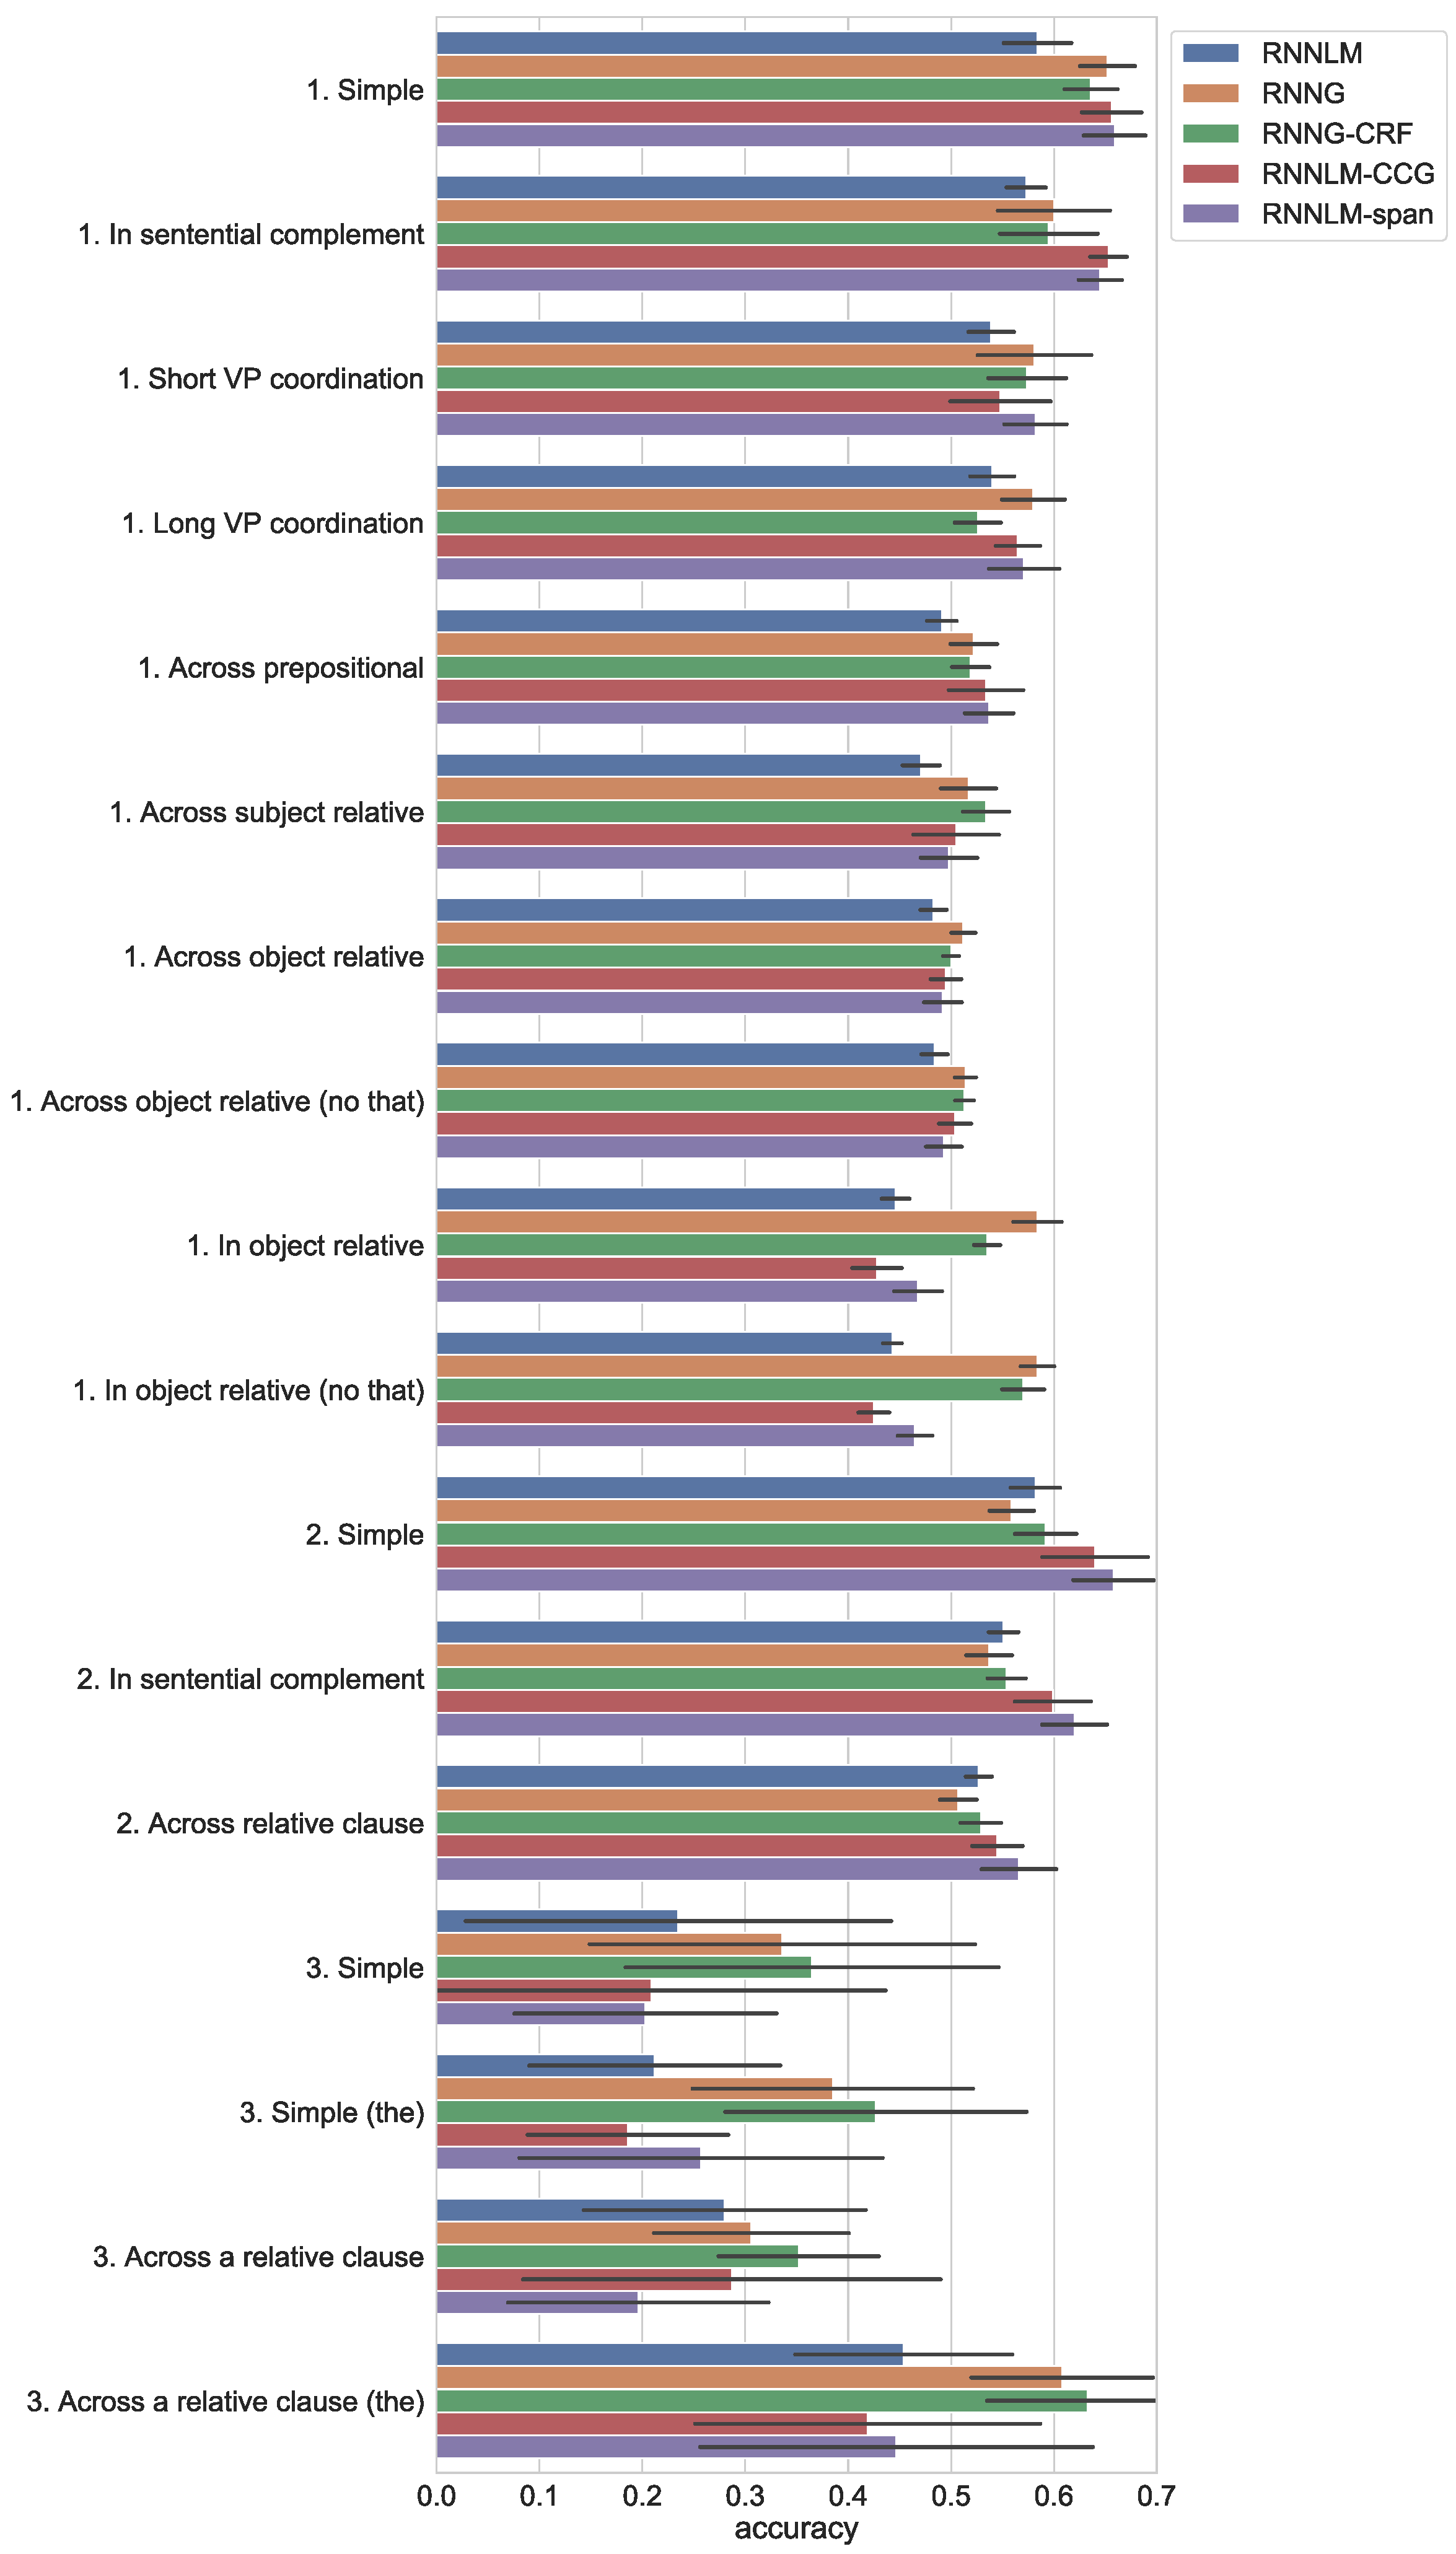
\includegraphics[width=\textwidth]{syneval/all_large-font.pdf}
      \caption{Syneval results for all models per category, bars showing standard deviation. The categories are described in appendix \ref{A5-syneval}.}
      \label{fig:syneval-all}
      \end{figure}
    \restoregeometry

    \begin{figure}[h]
      \center
      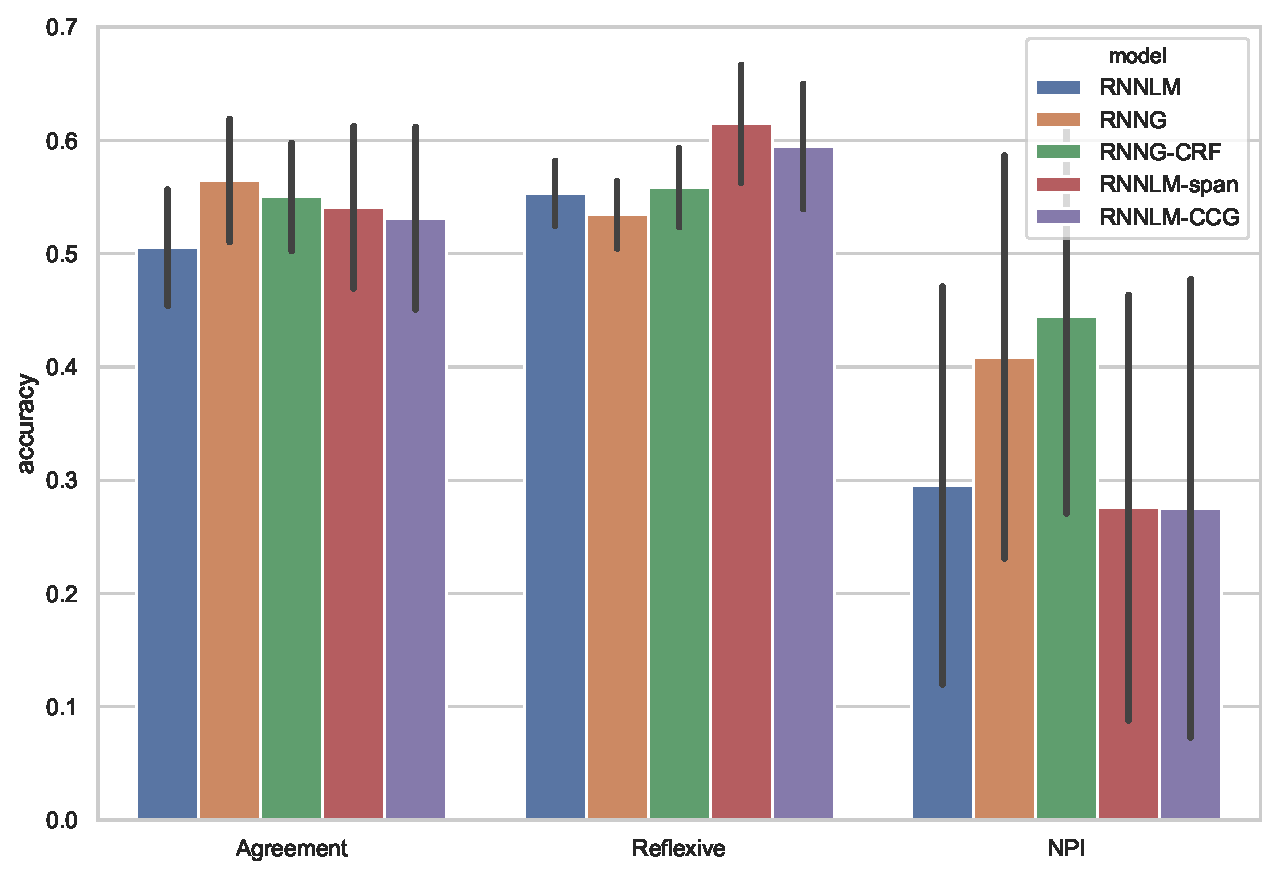
\includegraphics[width=0.9\textwidth]{syneval/all-averaged.pdf}
    \caption{Syneval results averaged over the three main categories.}
    \label{fig:syneval-all-averaged}
    \end{figure}

    \begin{figure}[h]
      \center
      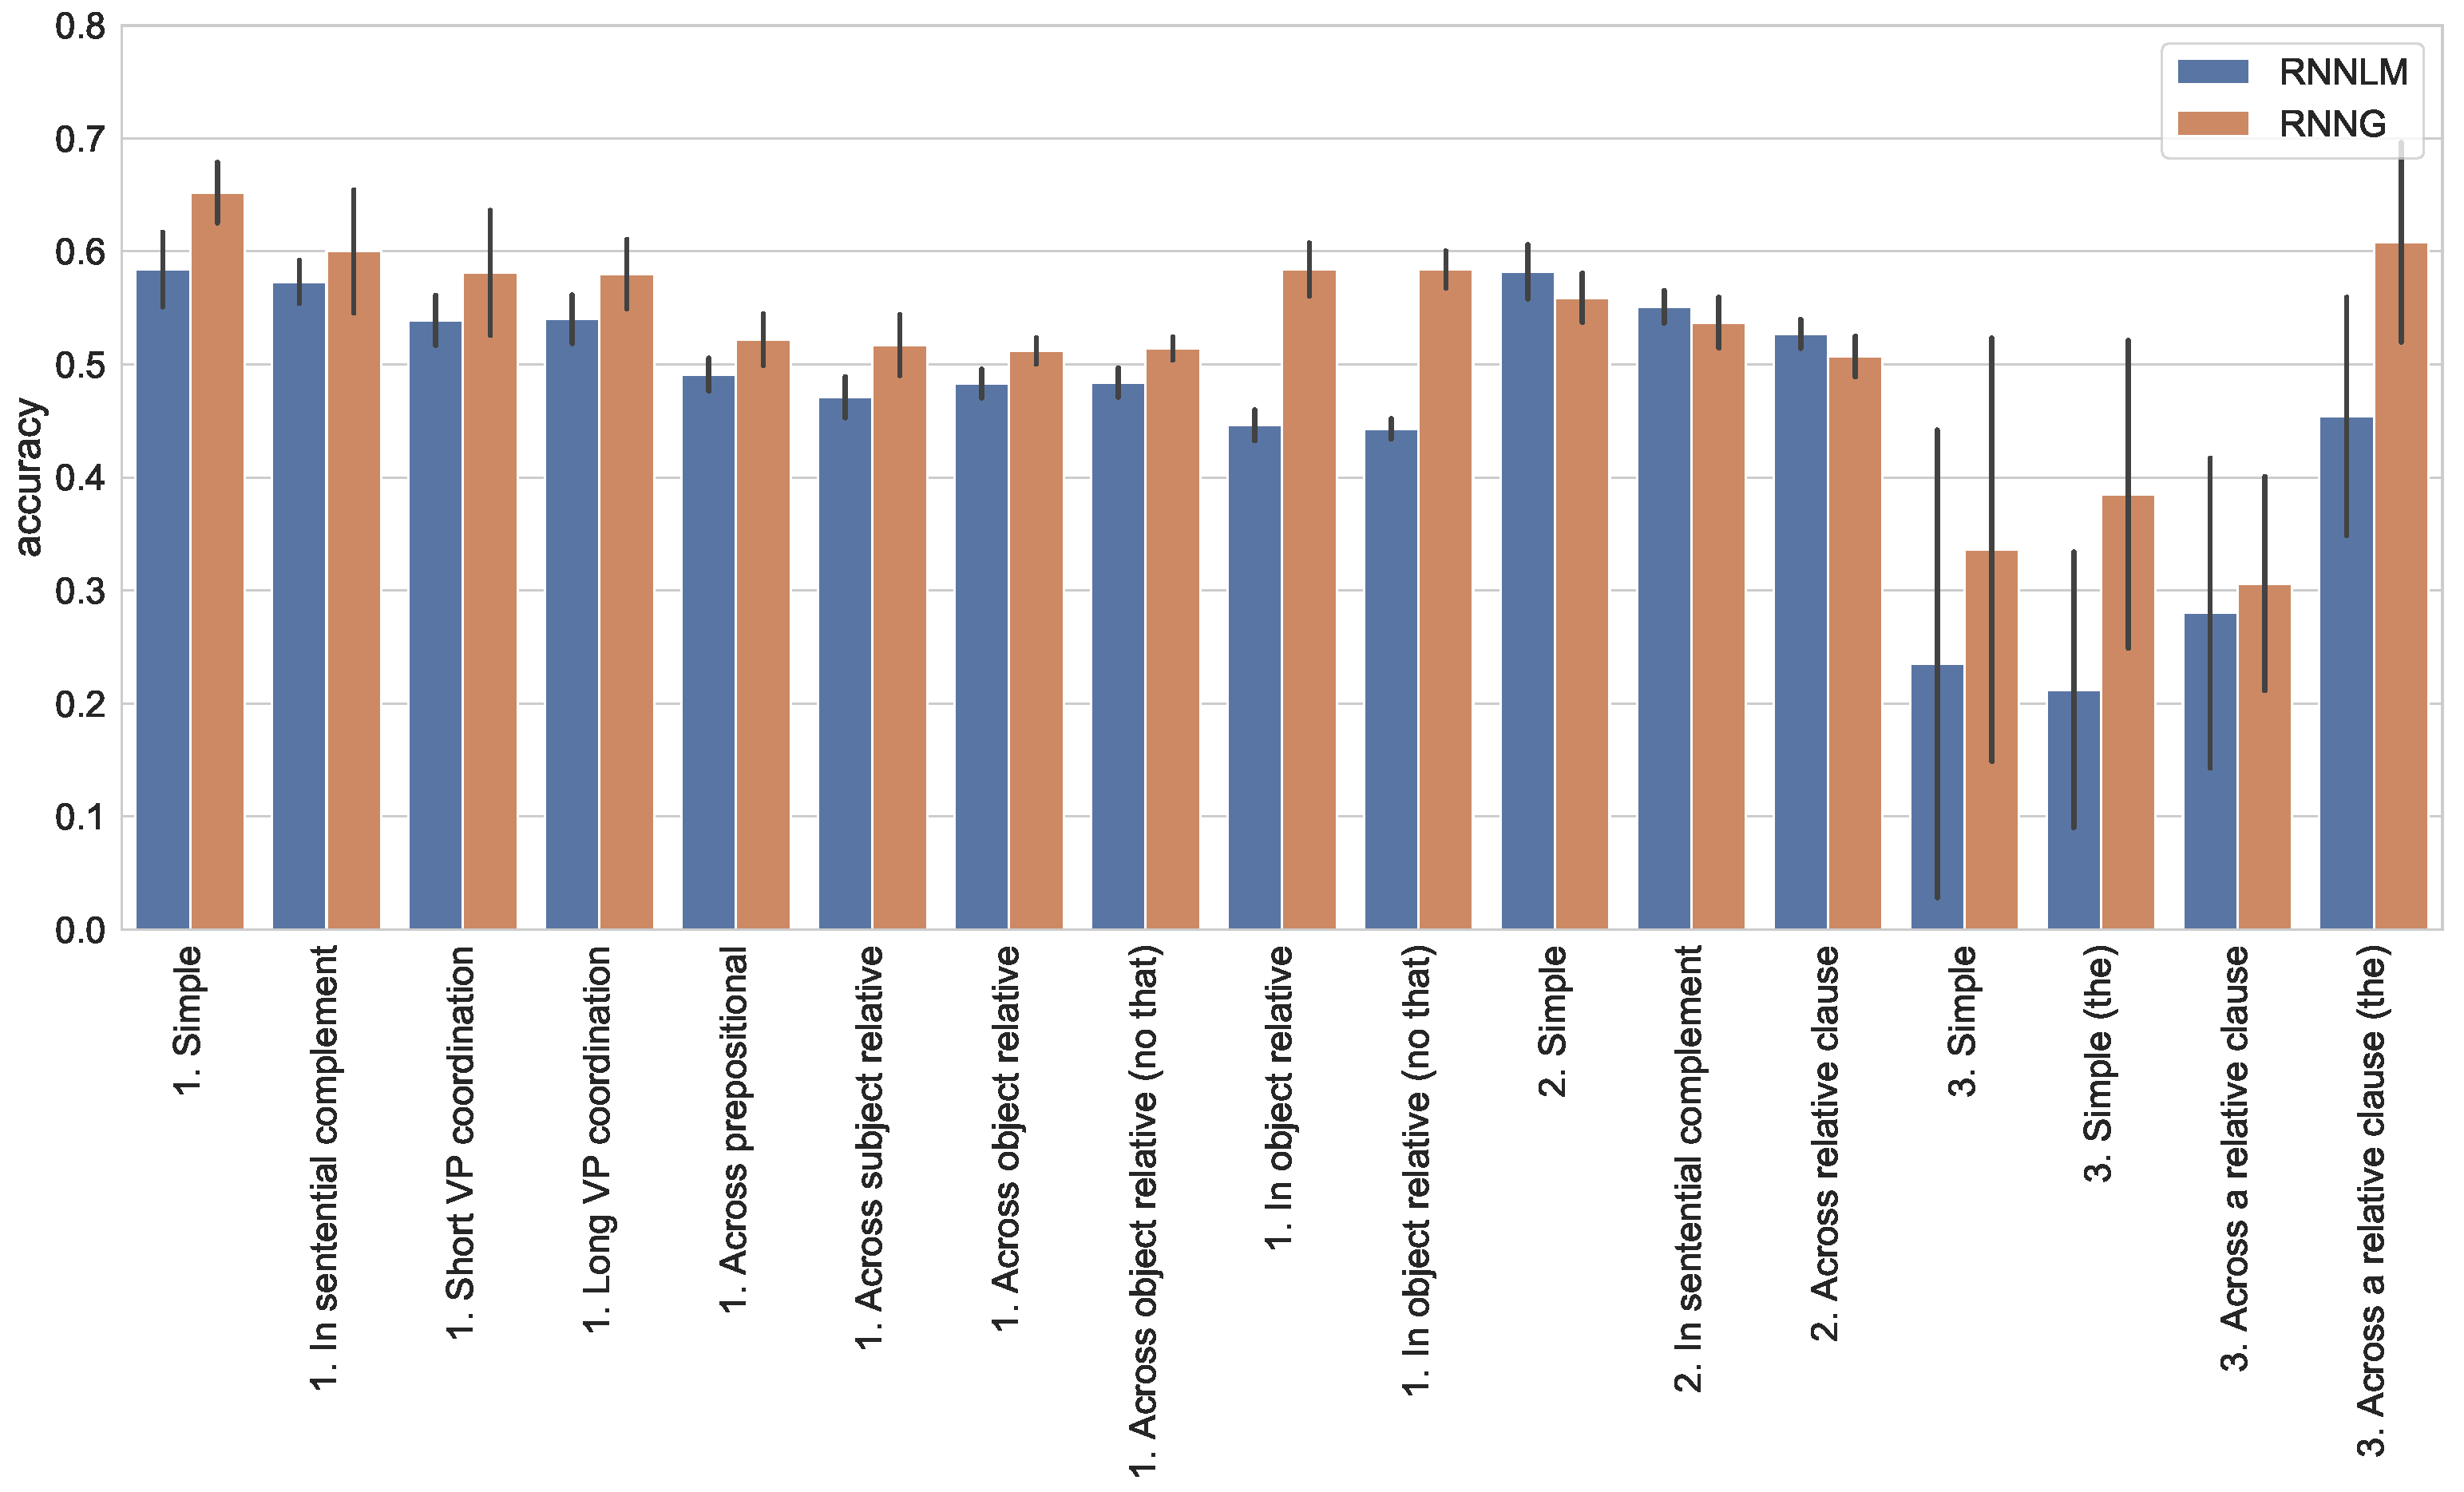
\includegraphics[width=\textwidth]{syneval/rnng_lm_horizontal.pdf}
    \caption{Syneval results for RNNLM and RNNG.}
    \label{fig:syneval-lm-rnng}
    \end{figure}

    \begin{figure}[h]
      \center
      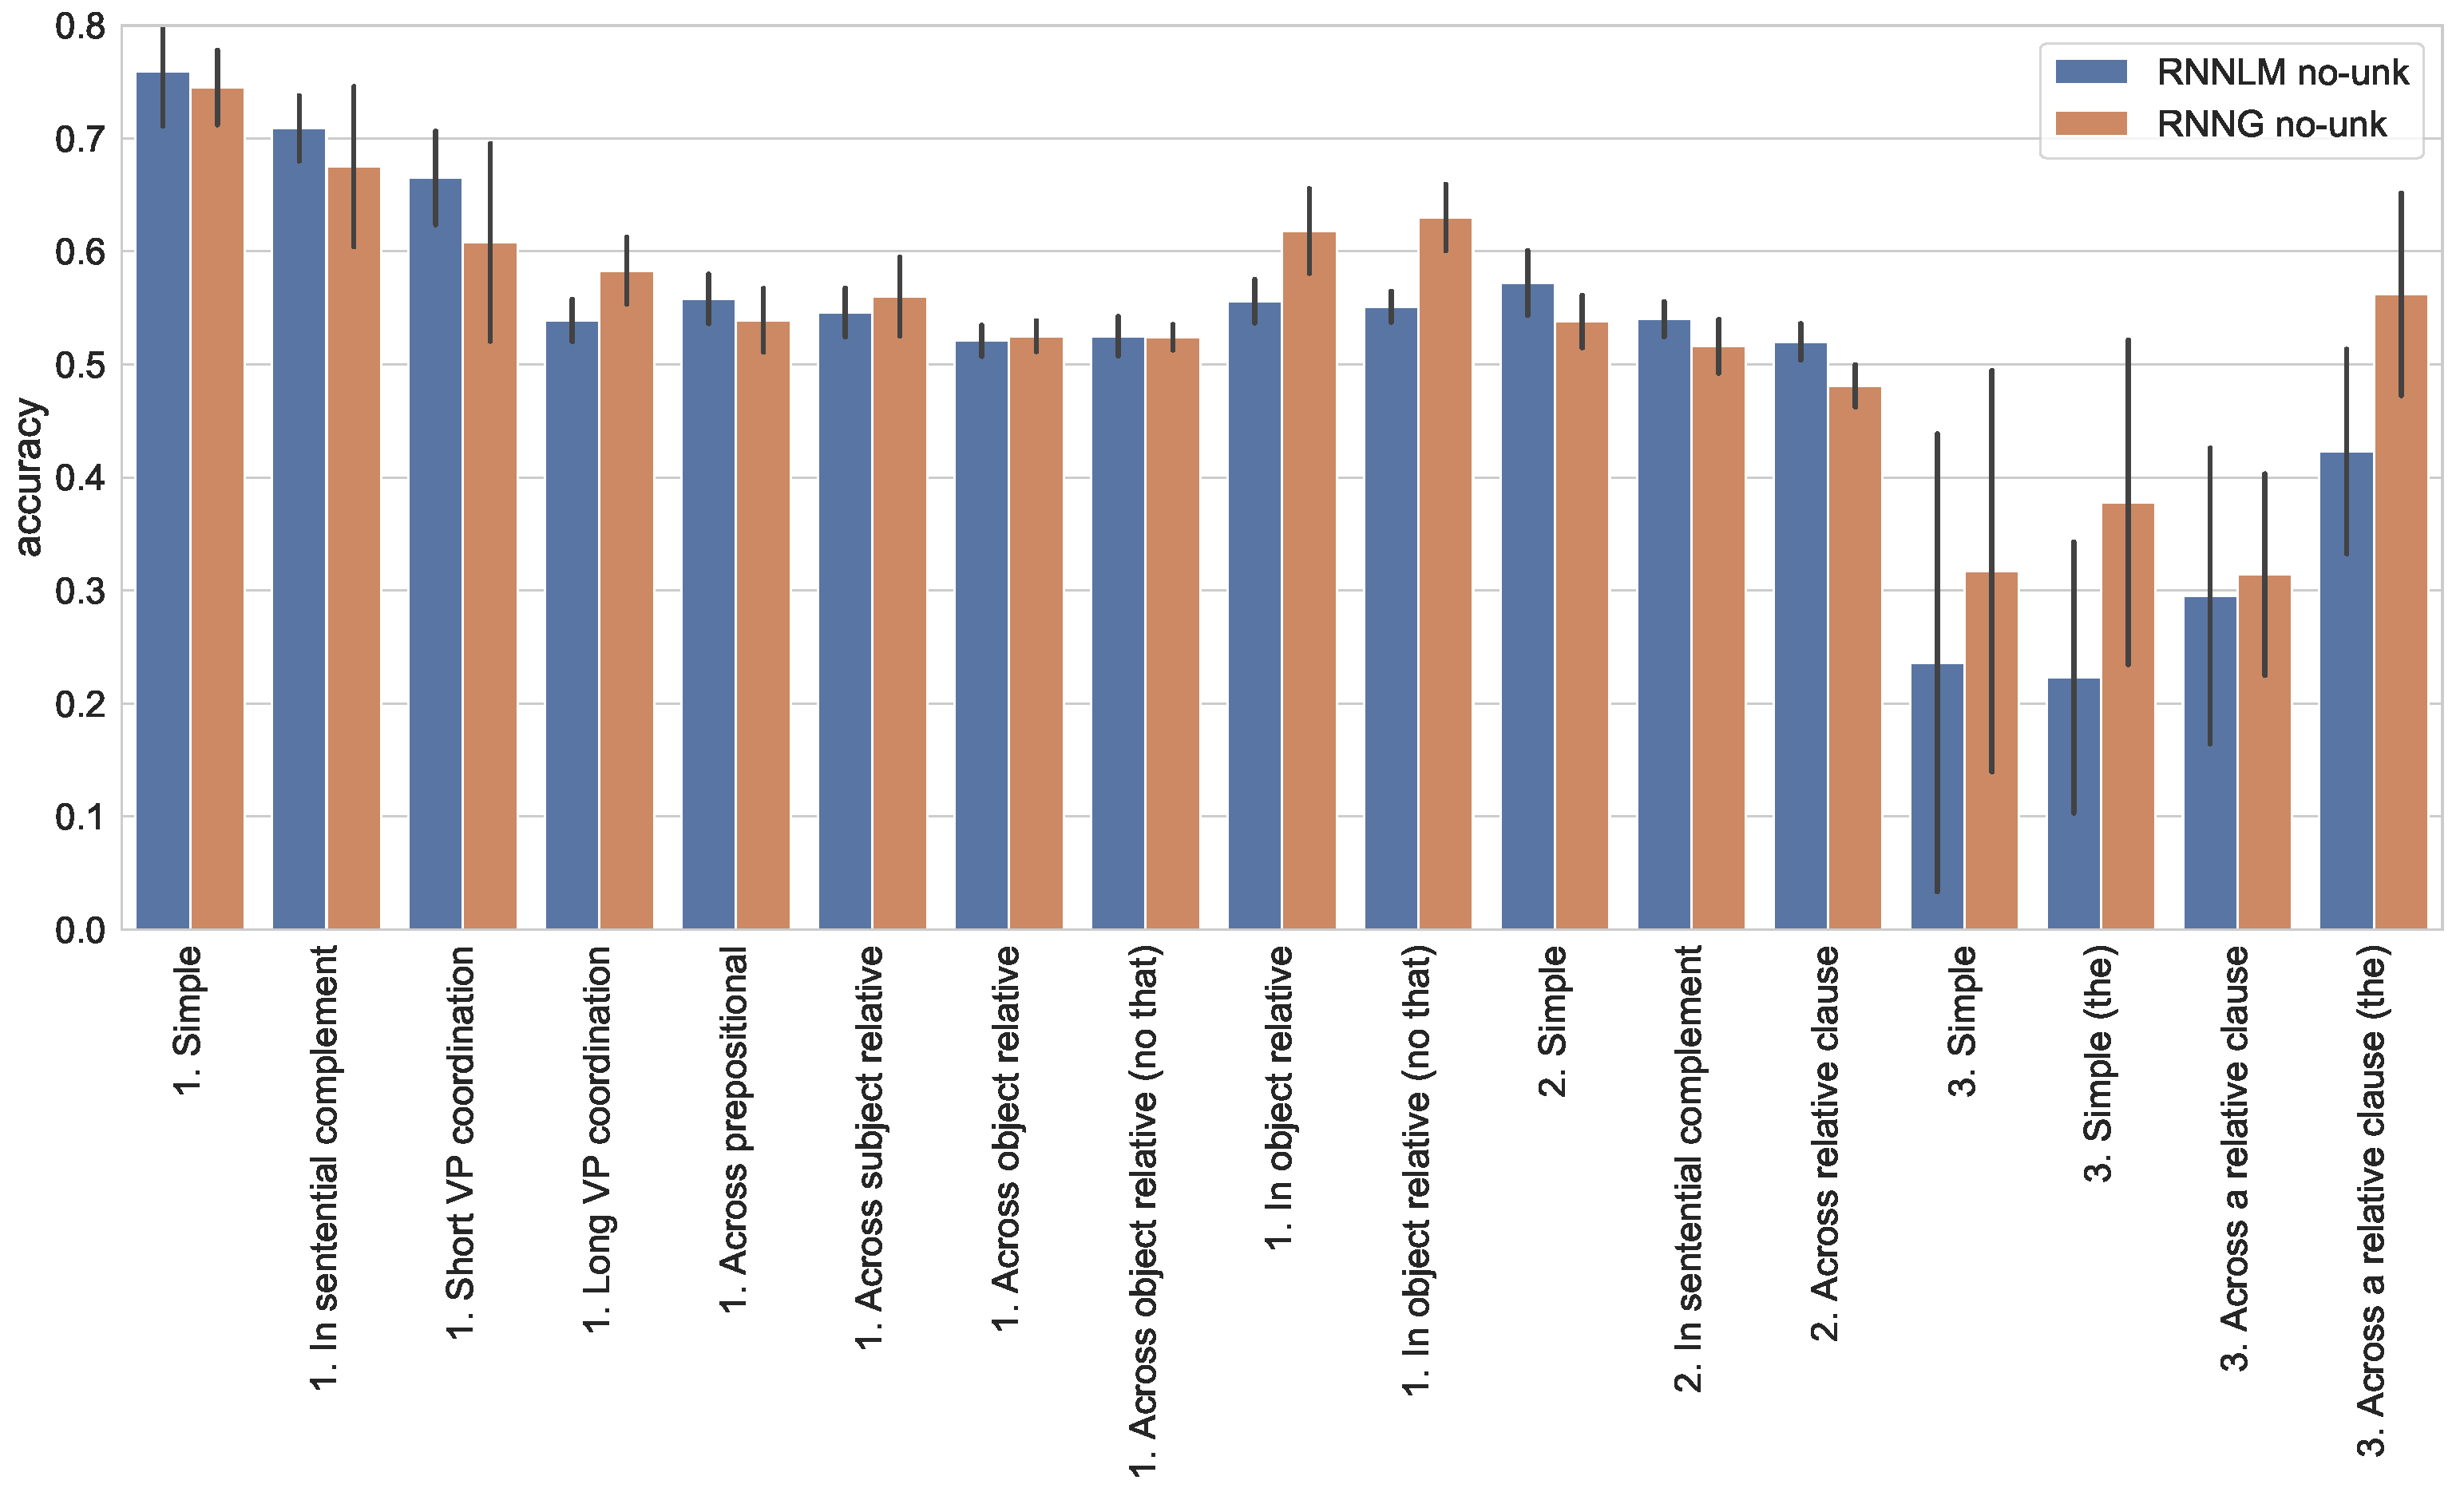
\includegraphics[width=\textwidth]{syneval/rnng_lm_no-unk_horizontal.pdf}
    \caption{Syneval results for RNNLM and RNNG, pairs with unknown words removed.}
    \label{fig:syneval-lm-rnng-nounk}
    \end{figure}

\section{Related work}
  There has been a surge recently of work on syntactic evaluation. \citet{linzen2016syntax} introduce the task of long distance subject-verb agreement and \citet{gulordava2018colorless} make this test more challenging by turning the sentences nonsensical while keeping them grammatical. Both datasets are extracted from a wikipedia corpus based on properties of their predicted dependency parse. To make the sentences nonsensical, \citet{gulordava2018colorless} randomly substitute words from the same grammatical category.\footnote{An approach inspired by Chomsky's (in)famous sentence \textit{Colorless green ideas sleep furiously} that is both grammatical and nonsensical.} \citet{warstadt2018acceptability} fine-tune neural models to learn to immitate grammatical acceptability judgments gathered from linguistics textbooks.

  \citet{mccoy2018revisiting} train a neural machine translation that turns a declarative sentence into a question, a kind of transformation that linguists have argued requires the existence of hierarchical structure in language \citep{everaert2015structures}.\footnote{Such declarative-question pairs play a central role as empirical evidence in the argument---known as the \textit{argument from the poverty of the stimulus}---that humans have an innate predisposition for generalizations that rely on hierarchical structure rather than linear order \citep{chomsky1980rules}.}

  Finally, targeted evaluation has been introduced previously for semantic comprehension by \citet{zweig2011microsoft} in a sentence completion task, and minimal contrastive sentence pairs have been used to evaluate neural machine translation by \citet{sennrich2017grammatical}.
